\chapter{Methodology}
\label{cp:methodology}

\section{Apparatus}\label{sec:apparatus}
\subsection{Airfoil Wake Measurements}
An airfoil is positioned in the wind tunnel test chamber as seen in \autoref{fig: AirFoilAndPressureRake}. Downstream of the airfoil is a pressure rake consisting \num{46} pressure taps, each spaced two millimeters apart. The pressure taps are connected to Scanivalve pressure transducers. A computer with data acquisition software collects measurements from the pressure transducers and stores the data in \verb|.csv| files.

\begin{figure}[htpb]
    \centering
    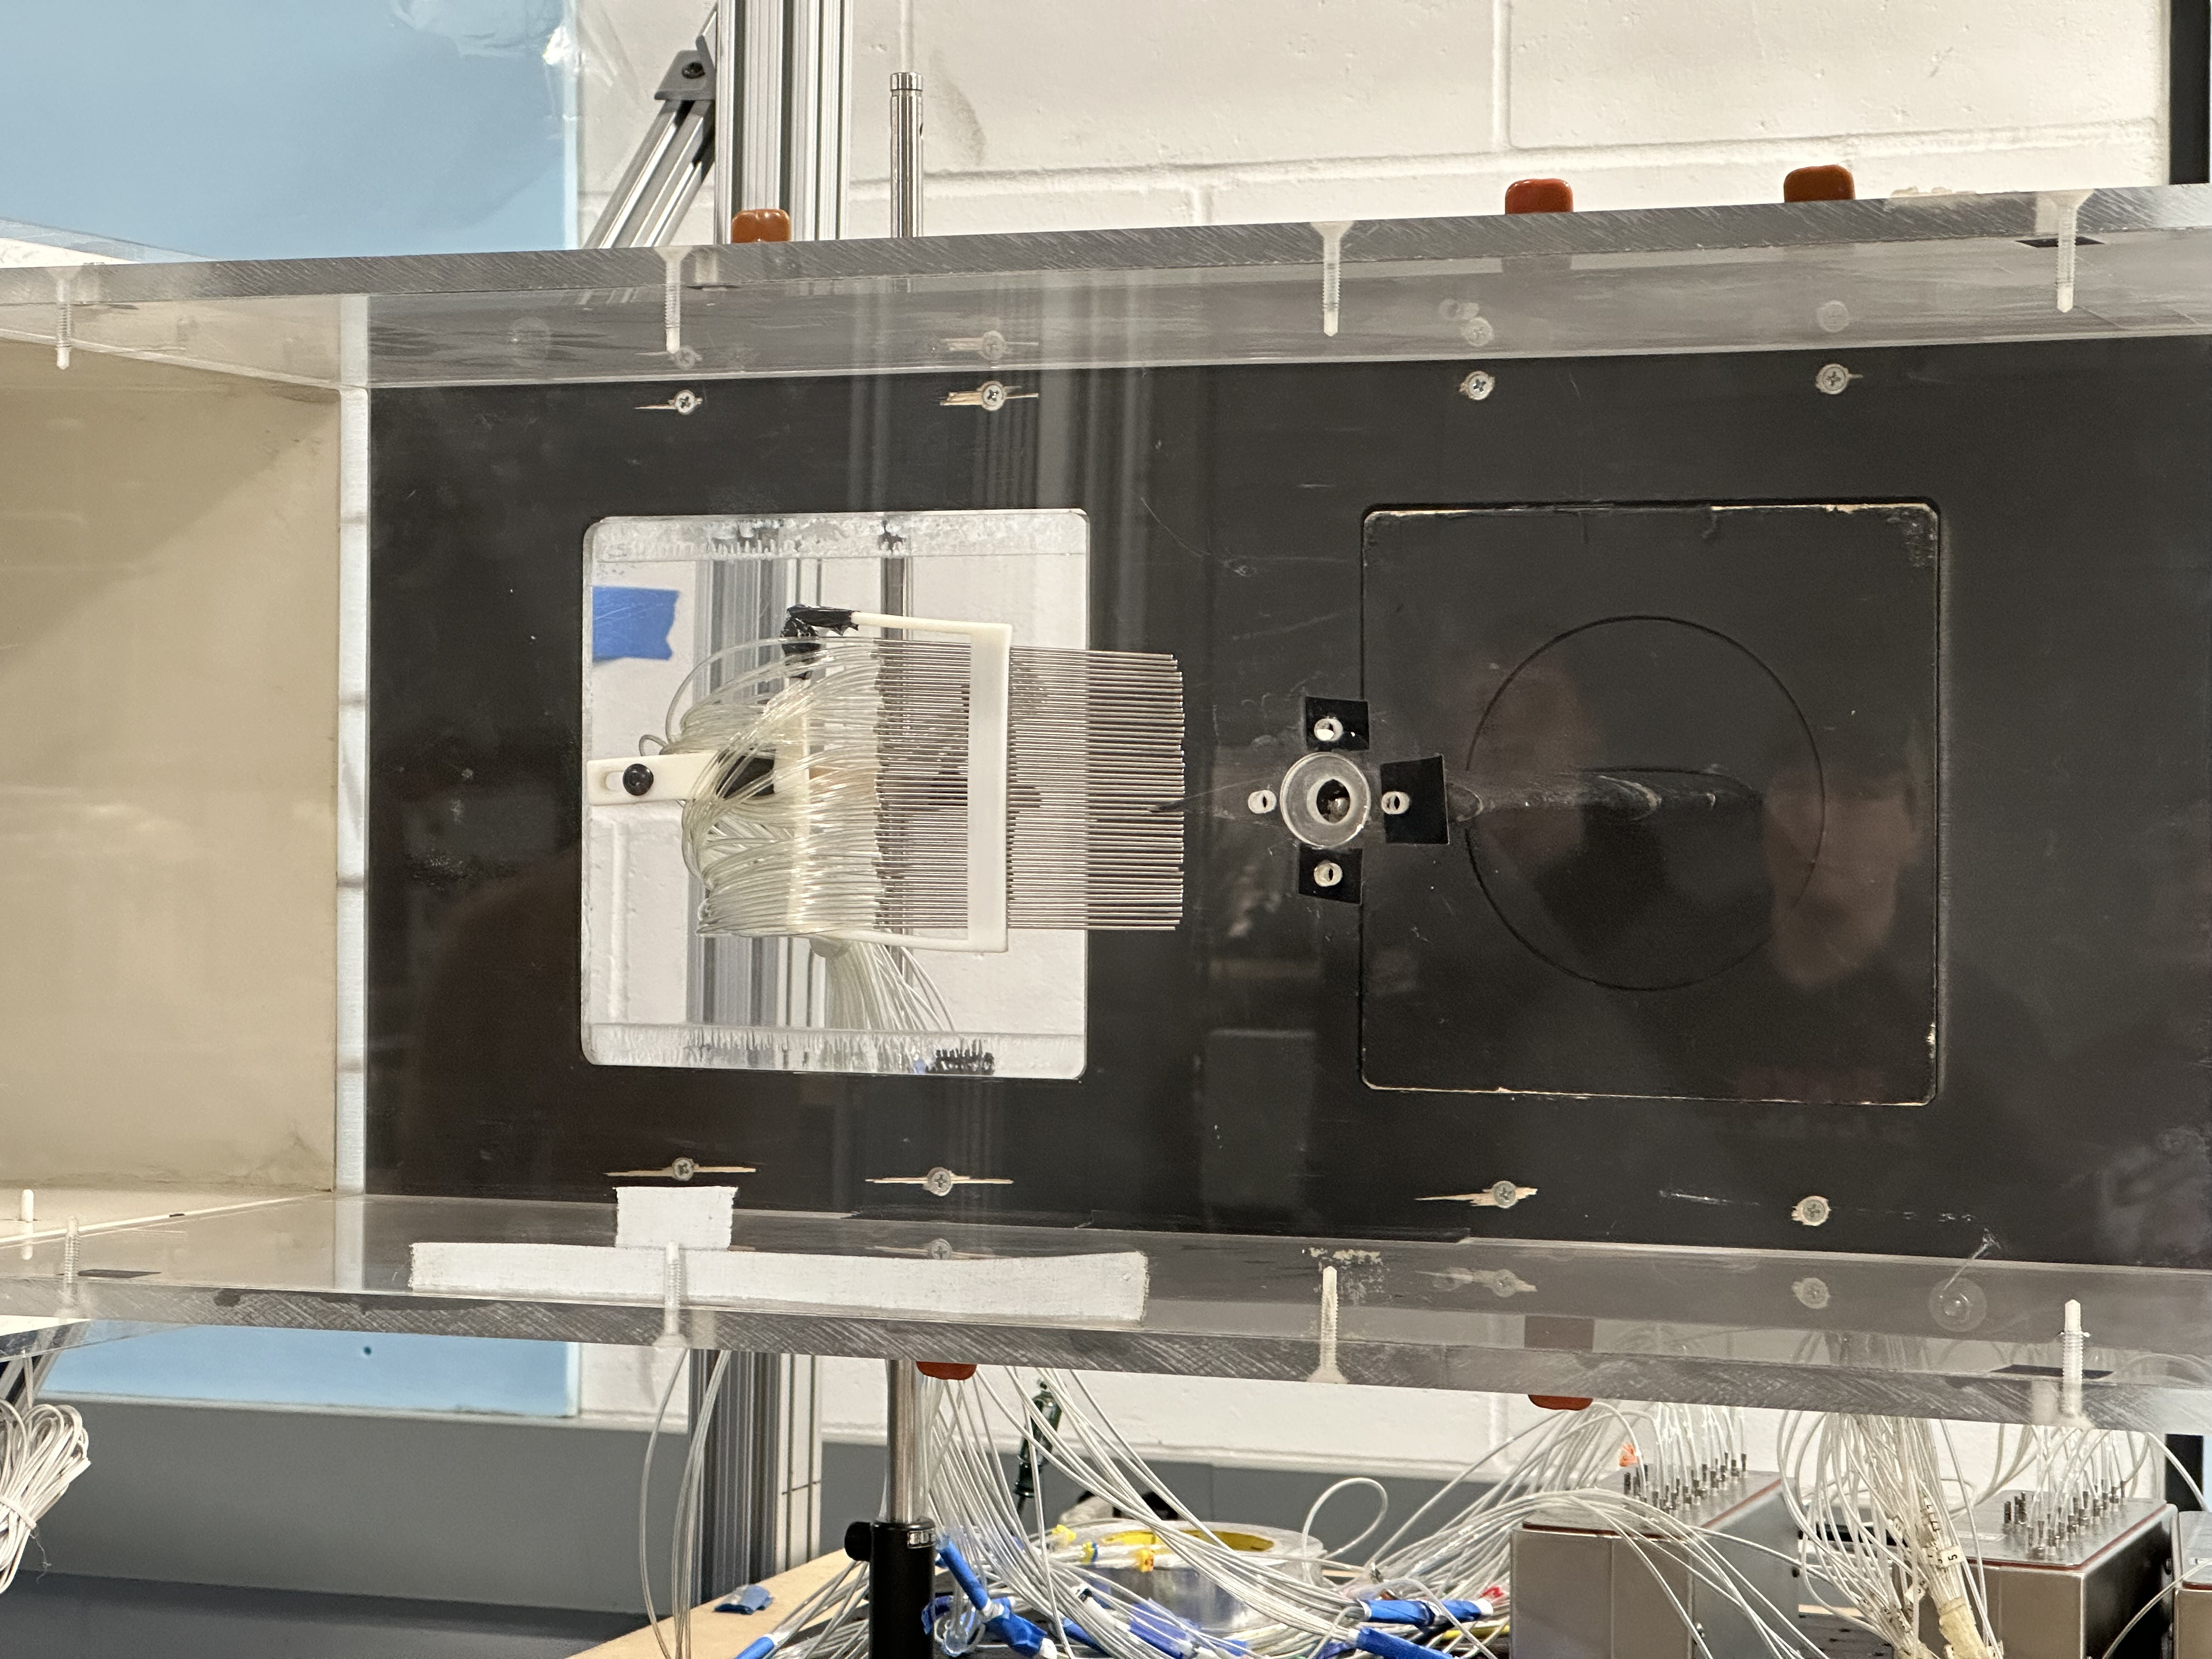
\includegraphics[width=0.75\linewidth]{Figures/IMG_3196.jpeg}
    \caption[Image of Airfoil and The Pressure Rake in Test Section.]{Image of Airfoil and The Pressure Rake in Test Section.}
    \label{fig: AirFoilAndPressureRake}
\end{figure}

\subsection{Hot Wire Anemometer Calibration}
A hot wire anemometer and pitot tube are positioned in the test chamber of a small wind tunnel. The pitot tube is connected to a Mensor manometer. Both the anemometer and Mensor manometer are connected to a computer with data acquisition software to collect measurements and store the data in \verb|.txt| files. 

\begin{figure}[htpb]
    \centering
    \includegraphics[width=0.75\linewidth]{Figures/IMG_3192.jpeg}
    \caption[Image of the small open Circuit wind tunnel.]{Image of the small open Circuit wind tunnel.}
    \label{fig: AirFoilAndPressureRake}
\end{figure}

\newpage
\section{Procedure}\label{sec:procedures}
\subsection{Airfoil Wake Measurements}
\begin{enumerate}
\item Calibrate the instruments with the wind tunnel set at 0 Hz.
\item Set the wind tunnel velocity at 10~15 Hz. Wait for velocity to become relatively uniform. 
\item Set the AOA to -4 degrees. 
\item Move the rake to cover the entire wake of the airfoil as necessary.
\item Acquire and save the data to a data file.
\item Repeat steps 3-4 for using the following AOAs: 0,4,6,8,10,12, and 16.
\item Save the data to a flash drive for past-lab analysis.
\end{enumerate}

\subsection{Hot Wire Anemometer Calibration}

\begin{enumerate}
\item Set the velocity to 0. \item Record data, including both the voltage data given by the computer and the presure data obtained from the mensor manometer.
\item Set the wind tunnel to 5 Hz and record data. 
\item Repeat step 2-3, from 5 Hz to 35 Hz, in increments of 5 Hz. 
\item Approximate the data to a 4th degree function. 
\item Save the data to a flash drive for post-lab analysis.
\end{enumerate}

\newpage
\section{Derivations}
The coefficient of pressure is found by normalizing the dynamic pressure measured by the pressure taps with the free-stream dynamic pressure. The difference between the inlet and outlet pressure of the contraction section, $P_A$ and $P_E$ respectively, along with the wind tunnel calibration constant, K, determines the free-stream dynamic pressure denoted as $q_\infty$.
\begin{equation}\label{eq:q_inf}
    q_\infty = K (P_A - P_E)
\end{equation}
The dynamic pressure at a singular tap from the pressure rake, generically described as the $i$th tap, is found by subtracting the total pressure measured by the tap with the free-stream static pressure.
\begin{equation}\label{eq:q_i}
    q_i = P_i - P_E 
\end{equation}
Therefore, the coefficient of pressure is can be by dividing \autoref{eq:q_i} by \autoref{eq:q_inf}:
\begin{equation}\label{eq:C_P}
    C_P = \frac{q_i}{q_\infty} = \frac{P_i - P_E }{K (P_A - P_E)}
\end{equation}
To begin calculations on the coefficient of drag, the flow velocity at each pressure tap is found by rearranging the generic dynamic pressure equation, $q = \frac{1}{2}\rho V^2$.
\begin{equation}\label{eq:U_i}
    U_i = \sqrt{\frac{2 q_i}{\rho}} = \sqrt{\frac{2 (P_i - P_E)}{\rho}}
\end{equation}
The free-stream flow velocity is found similarly: 
\begin{equation}\label{eq:U_inf}
    U_\infty = \sqrt{\frac{2 q_\infty}{\rho}} = \sqrt{\frac{2 K (P_A - P_E)}{\rho}}
\end{equation}
The coefficient of drag is found by looking at the fluid momentum change as drag resulting in \autoref{eq:C_D}, where $C$ is the chord of the airfoil and $y$ is the area downstream of the airfoil.
\begin{equation}\label{eq:C_D}
    C_D = \frac{2}{C} \int [\frac{U_y}{U_\infty}(1-\frac{U_y}{U_\infty})]dy
\end{equation}
Using 